\documentclass[12pt]{article}
\usepackage[a4paper, total={7.5in, 10in}]{geometry}
%\usepackage{array}
\usepackage{graphicx, subfig, wrapfig, fancyhdr, lastpage }
\newcommand\headerMe[2]{\noindent{}#1\hfill#2}
\usepackage[mathscr]{euscript}



\pagestyle{fancy}
\fancyhf{}

\rfoot{\em{Page \thepage \hspace{1pt} / \pageref{LastPage}}}
\begin{document}

\headerMe{Royaume du Maroc}{année scolaire \emph{2021-2022}}\\
\headerMe{Ministère de l'Éducation nationale, }{  Professeur :\emph{Zakaria Haouzan}}\\
\headerMe{du Préscolaire et des Sports}{Établissement : \emph{Lycée SKHOR qualifiant}}\\

\begin{center}
Devoir surveillé N°2 \\
    1BAC Sciences Mathématiques\\
Durée 2h00
\\
    \vspace{.2cm}
\hrulefill
\Large{Chimie 7pts}
\hrulefill\\

    \emph{Les deux parties sont indépendantes}
\end{center}
%end Headerss------------------------

\section*{Partie 1 : Les solutions électrolytiques\dotfill(4pts) }
Un flacon de déboucheur pour évier porte les indications suivantes :
   \begin{itemize}
      \item Produit corrosif.
      \item Contient de l’hydroxyde de sodium (soude caustique)., $\rho = 1000g/L$ , M(NaOH) = 60g/mol
      \item d=1,2 ,  Solution à 20\%.
   \end{itemize}
Le pourcentage indiqué représente le pourcentage massique d’hydroxyde de sodium (NaOH) contenu dans
le produit.
\begin{enumerate}
    \item Calculer la masse d’hydroxyde de sodium contenu dans $500 mL$ de produit.\dotfill(1pt)
    \item En déduire la concentration $C_0$ en soluté hydroxyde de sodium de la solution commerciale.\dotfill(0.5pt)
    \item On désire préparer un volume $V_1$ de solution $S_1$ de déboucheur 20 fois moins concentré que la solution commerciale.

        \begin{enumerate}
            \item Quelle est la valeur de la concentration $C_1$ de la solution ?\dotfill(1pt)
            \item Quelle est la quantité de matière d’hydroxyde de sodium contenu dans $250 mL$ de solution $S_1$?\dotfill(0.5pt)
            \item Quel volume de solution commerciale a-t-il fallu prélever pour avoir cette quantité de matière d’hydroxyde de sodium ?\dotfill(1pt)
        \end{enumerate}
\end{enumerate}

\section*{Partie 2 : Suivi d’une transformation chimique \dotfill(2pts)}
Le cuivre peut être préparé à partir du minerai constitué d’oxyde de cuivre (II) de formule CuO (s). On fait
réagir ce minerai avec du carbone C(s) (ou charbon de bois). Cette réaction produit du cuivre métallique Cu(s)
et du dioxyde de carbone. Les conditions initiales sont:$ m(CuO)_{(s)} = 9.85.10^2g$ et $m(C)_{(s)}=16.8g$. 
\begin{enumerate}
    \item Écrire l’équation de la réaction puis dresser le tableau d’avancement .\dotfill(1pt)
    \item Déterminer la valeur de l’avancement maximal $x_{max}$ et le réactif limitant.\dotfill(0.5pt)
    \item Réaliser un bilan de matière dans l’état final.\dotfill(0.5pt)

        \end{enumerate}
Données : $M(C) = 12,0 g.mol^{-1} ; M(CuO) = 79,5 g.mol^{-1} ; M(Cu) = 63,5 g.mol^{-1}$


%_____________________________________PHYSIque Partie 22222____________________________________________________________________________
\begin{center}
    \vspace{1cm}
\hrulefill
\Large{Physique 14pts}
\hrulefill\\
    \emph{Les Trois parties sont indépendantes}
\end{center}
%end Headerss------------------------
%_________________partie 2  : gravitation universelle :)

\section*{Partie 2 : Travail mécanique et énergie (11pts)}
\begin{wrapfigure}{r}{0.3\textwidth}

    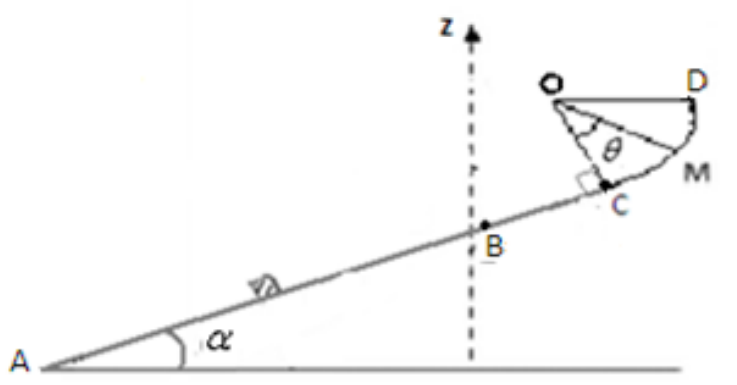
\includegraphics[width=0.3\textwidth]{./img/img01.png}
\end{wrapfigure}
Un corps solide S de masse m=0,4kg monte le long d’un rail composé de

-\underline{Une partie AB} rectiligne de longueur AB=1m et inclinée d’un angle $\alpha = 30^{\circ}$ par rapport à l’horizontale.

-\underline{Une partie BC} rectiligne de longueur BC=0,6m et inclinée d’un angle $\alpha = 30^{\circ}$ par rapport à l’horizontale.

-\underline{Une partie CD} circulaire de rayon r= 0,4m de centre O , son rayon OC $\perp$ BC. (voir schéma).

-\underline{Les frottements sont négligeables} sur AB et CD et on les considère équivalents à une force constante $\vec{f}$ sur la partie BC.

\begin{enumerate}
    \item On applique sur le corps S une force $\vec{F}$ constante et parallèle à la ligne de plus grande pente et il part du point A sans vitesse initiale et arrive au point B avec une vitesse $V_B$=4 m/s.
        \begin{enumerate}
            \item Faire le bilan des forces qui s’exercent sur le corps S sur la partie AB.\dotfill(1pt)
            \item Donner l’énoncé du théorème de l’énergie cinétique.\dotfill(1pt)
            \item En appliquant le théorème de l’énergie cinétique sur S entre A et B déterminer l’intensité de la force $\vec{F}$.\dotfill(1pt)
        \end{enumerate}
        \item Au point B on élimine la force $\vec{F}$ et le corps S continue son mouvement sur la partie BC du trajet et passe par le point C avec une vitesse $V_c$=1,3m/s .On considère le plan horizontal passant par le point B comme état de référence pour l’énergie potentielle de pesanteur.
            \begin{enumerate}
                \item  Donner la variation de l’énergie potentielle de pesanteur du corps S entre B et C. \dotfill(1pt)
                \item Donner l’expression de la variation de l’énergie mécanique du corps S entre B et C.\dotfill(1pt)
                \item En déduire la valeur de l’intensité de la force de frottement $\vec{f}$\dotfill(1pt)
            \end{enumerate}

            \item Le corps S continue son mouvement sur la partie CD sans frottement pour arriver au point M avec une vitesse nulle.
                \begin{enumerate}
                    \item Déterminer l’énergie mécanique du corps S au point C.\dotfill(1pt)
                    \item Monter que l’expression de l’énergie mécanique du corps S au point M s’écrit :\dotfill(2pts)

                        $${E_m}_M = mg.(BC.sin\alpha + r[cos\alpha - cos(\alpha + \theta)])$$                    \item En appliquant la loi de conservation de l’énergie mécanique, déterminer la valeur de l’angle $\theta$...\dotfill(2pt)
                \end{enumerate}
\end{enumerate}
On donne : g=10N/kg

\section*{Partie 3 :Mode de transfert d’énergie (3pts)}

Si-Brahim a lancé une bille verticalement vers le haut à une altitude
h = 1,5m par rapport au sol, avec une vitesse $V_A= 10 m/s$.
On considère que le poids est la seule force appliquée à la
bille (chute libre).
On donne $g = 10 N/kg$.
Calculer en utilisant le théorème de l’énergie cinétique :

   1. La hauteur maximale atteinte par la bille.

   2. La vitesse de la bille lorsqu’elle retombe sur le sol.


\end{document}
